\documentclass[conference]{IEEEtran}
\IEEEoverridecommandlockouts
\usepackage{cite}
\usepackage{amsmath,amssymb,amsfonts}
\usepackage{algorithmic}
\usepackage{graphicx}
\usepackage{textcomp}
\usepackage{xcolor}
\usepackage{booktabs}
\usepackage{tikz}
\usetikzlibrary{arrows.meta,positioning,fit}
\graphicspath{{figures/}}
\def\BibTeX{{\rm B\kern-.05em{\sc i\kern-.025em b}\kern-.08em
    T\kern-.1667em\lower.7ex\hbox{E}\kern-.125emX}}

\begin{document}

\title{EmergencyFlow: A Reproducible Closed-Loop Simulation Testbed for Safety-Verified Emergency Vehicle Signal Priority}

% TODO: replace with the team's names, departments, institution and e-mail addresses.
\author{\IEEEauthorblockN{Author Name}
\IEEEauthorblockA{\textit{Department of Computer Engineering} \\
\textit{Institution Name}\\
Navi Mumbai, India \\
email address}
\and
\IEEEauthorblockN{Author Name}
\IEEEauthorblockA{\textit{Department of Computer Engineering} \\
\textit{Institution Name}\\
Navi Mumbai, India \\
email address}
\and
\IEEEauthorblockN{Author Name}
\IEEEauthorblockA{\textit{Department of Computer Engineering} \\
\textit{Institution Name}\\
Navi Mumbai, India \\
email address}
\and
\IEEEauthorblockN{Author Name}
\IEEEauthorblockA{\textit{Department of Computer Engineering} \\
\textit{Institution Name}\\
Navi Mumbai, India \\
email address}
}

\maketitle

\begin{abstract}
Ambulances lose minutes at signalised junctions, and signal preemption is the classic remedy, yet claims about its benefit are hard to compare because evaluations differ in traffic, baselines and safety accounting. We present EmergencyFlow, an open simulation testbed that closes the loop between a microscopic traffic simulator, a rule-based decision layer, an independently verified safety layer and an interactive three-dimensional view in which a person drives the ambulance. Every signal action passes a safety controller that replays it against the junction conflict matrix and minimum clearance times, and a separate monitor checks the signal states actually produced by the simulator at every step. The same engine runs headless for evaluation: eight arms combining three signal strategies, a red-crossing baseline and two routing policies are compared on identical, seeded traffic, against a fixed-time program tuned for each demand level so the baseline is not a strawman. Over 560 paired runs on a sixteen-junction grid, preemption cut mean ambulance travel time from 197 to 94 seconds at heavy demand with no measurable change in background delay and no signal-safety violation, while crossing red lights without priority saved far less time and caused junction collisions. Queue-aware coordination and live re-routing gave no further measurable gain without incidents. A live shadow simulation replays each mission with normal signals, so the time saved is measured on the same traffic rather than estimated.
\end{abstract}

\begin{IEEEkeywords}
emergency vehicle preemption, traffic signal control, SUMO, microscopic traffic simulation, safety verification, reproducible evaluation, human in the loop
\end{IEEEkeywords}

\section{Introduction}

Emergency medical response is a race against time, and in dense urban networks a large share of an ambulance's delay is spent waiting at signalised junctions or behind queues that formed during red. Emergency vehicle preemption (EVP), which switches the next signal to green for the approaching vehicle, has been deployed for decades \cite{fhwa_evp}. Its benefit is usually reported from field trials or from simulations built for a single study, which makes results difficult to reproduce and to compare: the traffic differs between runs, the baseline signal plan is rarely tuned, and the cost to other road users and the safety of the switching itself are often reported loosely or not at all.

This paper describes EmergencyFlow, a simulation testbed built to make such comparisons fair and inspectable. Its design follows four principles. First, the traffic simulator is the single source of truth: SUMO \cite{sumo} computes every vehicle position, speed and signal state, and the user interface only renders and sends intent. Second, decision logic proposes and a safety layer disposes: no rule may actuate a signal directly. Third, safety is verified twice, by the controller before an action and by an independent monitor on the states the simulator actually produced. Fourth, every claim is measured on paired, seeded runs, with the baseline given the best fixed-time program for its demand.

The contributions are:
\begin{itemize}
\item a closed-loop architecture coupling SUMO, a Python decision and safety engine and a browser-based 3D view in which a human drives the ambulance, with one simulation thread owning the simulator connection;
\item a safety controller and an independent monitor that enforce conflict-free greens and minimum yellow and all-red clearance, with every decision logged with its reason;
\item a paired evaluation methodology with demand-tuned baselines, a red-crossing baseline, exact Wilcoxon tests and bootstrap confidence intervals, and collision attribution by deterministic replay;
\item results from 560 runs showing large, robust travel-time gains from preemption at no measurable background cost, and no measured benefit from coordination or live re-routing in the absence of incidents;
\item a live shadow simulation that measures, rather than estimates, the time saved by each interactive mission against normal signals.
\end{itemize}

The decision logic is deliberately rule-based. The testbed is a simulation and does not control real traffic signals.

\section{Related Work}

Signal preemption for emergency vehicles is a mature field practice; the U.S. Federal Highway Administration's cross-cutting study \cite{fhwa_evp} documents deployments, detection technologies and reported reductions in response time, and notes that safe transition through yellow and all-red intervals is essential. Clearance intervals of this kind are standardised in traffic control manuals \cite{mutcd}. Fixed-time plans are commonly dimensioned with Webster's method \cite{webster}, which minimises average delay for a given demand; we use SUMO's implementation of this method to tune the baseline.

Microscopic simulation is the standard tool for studying such strategies. SUMO \cite{sumo} provides car-following \cite{krauss} and lane-changing \cite{erdmann} models and exposes run-time control through the TraCI interface \cite{traci}. Many preemption studies use such simulators, but typically compare a strategy with an untuned baseline on unpaired traffic and report a single scenario. Our work does not propose a new preemption algorithm; its contribution is the closed-loop testbed, the verified safety layer and the evaluation protocol, which together allow strategies to be compared on equal terms. Route guidance for the ambulance uses a time-dependent shortest-path search in the spirit of Dijkstra's algorithm \cite{dijkstra}, and statistical comparisons follow standard paired non-parametric practice \cite{wilcoxon,efron,efron_book}.

\section{System Architecture}

Fig.~\ref{fig:arch} shows the three tiers. SUMO runs as a separate process and is the single source of truth. A Python engine connected through TraCI hosts the decision logic, the safety layer, routing and the experiment runner. A browser front end built with React and Three.js renders the city in 3D and sends user intent over a WebSocket.

\begin{figure}[t]
\centering
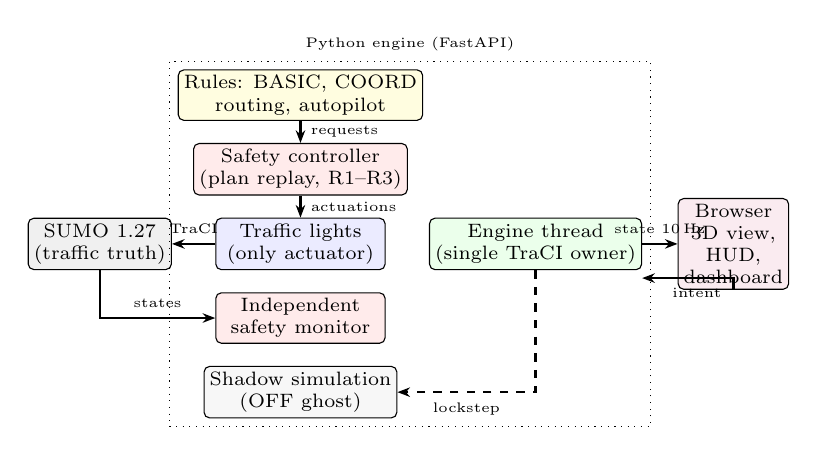
\begin{tikzpicture}[
  box/.style={draw, rounded corners=2pt, align=center, font=\scriptsize, minimum height=0.62cm, inner sep=2pt},
  arr/.style={-{Stealth[length=1.6mm]}, thick},
  lab/.style={font=\tiny, align=center}
]
\node[box, fill=gray!12, minimum width=1.7cm] (sumo) {SUMO 1.27\\(traffic truth)};
\node[box, fill=blue!8, right=0.55cm of sumo, minimum width=2.15cm] (tl) {Traffic lights\\(only actuator)};
\node[box, fill=red!8, above=0.28cm of tl, minimum width=2.15cm] (sc) {Safety controller\\(plan replay, R1--R3)};
\node[box, fill=yellow!12, above=0.28cm of sc, minimum width=2.15cm] (rules) {Rules: BASIC, COORD\\routing, autopilot};
\node[box, fill=red!8, below=0.28cm of tl, minimum width=2.15cm] (mon) {Independent\\safety monitor};
\node[box, fill=green!8, right=0.55cm of tl, minimum width=1.9cm] (eng) {Engine thread\\(single TraCI owner)};
\node[box, fill=purple!8, right=0.45cm of eng, minimum width=1.25cm] (ui) {Browser\\3D view,\\HUD,\\dashboard};
\node[box, fill=gray!6, below=0.28cm of mon, minimum width=2.15cm] (ghost) {Shadow simulation\\(OFF ghost)};
\draw[arr] (rules) -- node[lab, right]{requests} (sc);
\draw[arr] (sc) -- node[lab, right]{actuations} (tl);
\draw[arr] (tl) -- node[lab, above]{TraCI} (sumo);
\draw[arr] (sumo.south) |- node[lab, pos=0.75, above]{states} (mon.west);
\draw[arr] (eng) -- node[lab, above]{state 10\,Hz} (ui);
\draw[arr] (ui.south) |- node[lab, pos=0.7, below]{intent} ([yshift=-1mm]eng.south east);
\draw[arr, dashed] (eng.south) |- node[lab, pos=0.75, below]{lockstep} (ghost.east);
\node[draw, dotted, inner sep=3pt, fit=(rules)(sc)(tl)(mon)(eng)(ghost), label={[font=\tiny]above:Python engine (FastAPI)}] {};
\end{tikzpicture}
\caption{Architecture. Decision rules only request; the safety controller turns accepted requests into actuations executed by the single traffic-light module; an independent monitor checks the states SUMO actually produced.}
\label{fig:arch}
\end{figure}

\subsection{Simulation Engine and Concurrency}

TraCI is not thread-safe, so one engine thread owns the connection. WebSocket handlers only submit commands, which the engine applies before each step. Each tick runs, in order: queued commands; manual or autopilot control of the ambulance; the safety controller's step and its actuations; one simulation step of 0.1\,s; observation of the ambulance; the safety monitor; the preemption rule; route re-planning; and publication of an immutable state, which the event loop serialises once and fans out to every client. Per-step reads use TraCI subscriptions rather than per-vehicle queries. In live mode the engine paces steps at 10\,Hz; on the evaluation grid at demand 1.5 with about 480 vehicles the median tick took 7.8\,ms (95th percentile 11.4\,ms), almost all of it in the simulator, well within the 100\,ms budget.

\subsection{Road Network and Traffic}

The scenarios are generated grids of signalised junctions 250\,m apart with 200\,m roads to the map edge, two lanes per direction at 13.89\,m/s, and left-hand traffic. Each junction runs a fixed-time program with paired opposite approaches, a 4\,s yellow and a 2\,s all-red per change. Background demand is a set of Poisson flows between every pair of map-edge roads, 400 vehicles per hour per entry at demand 1.0, so the random seed changes the traffic. This paper's experiments use the $4\times4$ grid (16 junctions).

\subsection{Human in the Loop}

In the interactive mode a person drives the ambulance with the keyboard: throttle and brake, a turn choice for the next junction, and lane changes. These are intents, not physics. The engine checks their feasibility and applies them to the simulated vehicle, which keeps SUMO's safe-speed and right-of-way behaviour; a dead-man timer stops the vehicle if input stops for 0.5\,s. The 3D view interpolates between simulation ticks and never predicts motion. On the evaluation grid it rendered at the display's 144\,frames per second on a discrete laptop GPU and at a median of 60 on an integrated GPU, with a median of 45\,ms from key press to the first responding tick. A read-only dashboard can be opened from a second computer on the local network. Fig.~\ref{fig:live} shows the chase view.

\begin{figure}[t]
\centering
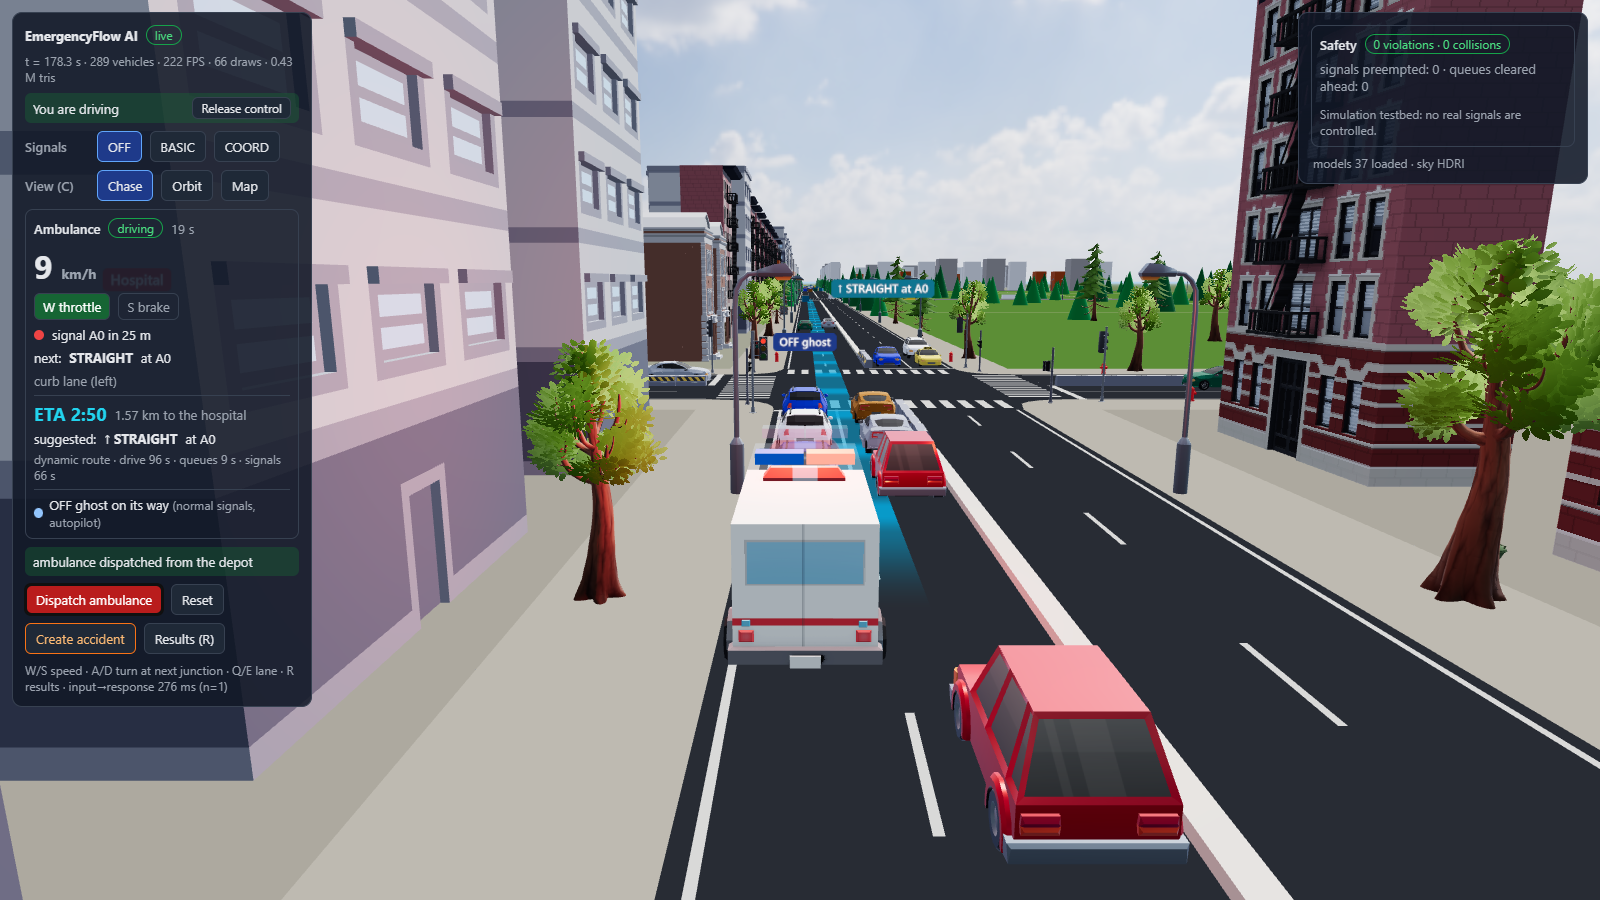
\includegraphics[width=\columnwidth]{live_chase_ghost.png}
\caption{Interactive chase view: the suggested route is drawn on the road, the HUD shows ETA, next signal and safety log, and the translucent ``OFF ghost'' marks where the same mission stands under normal signals.}
\label{fig:live}
\end{figure}

\section{Decision Logic and Safety Layer}

\subsection{Rule-Based Preemption (BASIC)}

The ambulance's next signal, the exact link it will use and its distance $d$ are read from the simulator. With speed $v$, the arrival estimate is
\begin{equation}
\mathrm{ETA} = \frac{d}{\max(v,\, 5\,\mathrm{m/s})},\label{eq:eta}
\end{equation}
where the floor keeps a slow or stopped ambulance near the stop line eligible. When $\mathrm{ETA}\le 15$\,s, BASIC requests the approach-exclusive state, in which every link from the ambulance's incoming road is green and every other link red. Links losing green show yellow for 4\,s and then an all-red of 2\,s. A preemption is released once the ambulance has passed the junction, and it times out after 40\,s. Recovery runs the same clearance and resumes the normal program at the other direction's green, which then holds for at least 10\,s before the junction accepts a new preemption.

\subsection{Queue-Aware Coordination (COORD)}

COORD adds two rule-based elements. First, the lead time grows with the queue in front of the ambulance, so that the queue has discharged before it arrives:
\begin{equation}
\mathrm{ETA}\le \min\!\left(30,\; c + s + \frac{q}{n}\,h + m\right),\label{eq:lead}
\end{equation}
with clearance $c=6$\,s, start-up loss $s=2$\,s, $q$ halted vehicles over $n$ lanes, headway $h=2$\,s and margin $m=3$\,s; the 30\,s cap keeps the hold within the 40\,s limit. Second, the same rule is applied to the next three signalised junctions along the suggested route, preparing them in advance.

\subsection{Routing}

Routes are planned by a time-dependent shortest-path search over a graph whose nodes are roads and whose arcs are junction movements. The cost of a route is its predicted travel time: driving time at the ambulance's speed or the speed of moving traffic, the loss of a standing start, queue discharge at 2\,s per halted vehicle and lane, the expected signal wait (predicted from the fixed-time program under normal signals, residual under preemption), small turn penalties, and an accident penalty. Live queues and exact signal timing are used only for the next 30\,s, beyond which expected values take over. The route is re-planned every second and on every new road, and a new suggestion replaces the current one only if it is faster by at least $\max(5\,\mathrm{s},\,10\,\%)$. In the interactive mode routing is advisory and never steers. Over ten seeded runs the predicted ETA at dispatch had a mean absolute error of 11\,s (10\,\%) with preemption and 42\,s (25\,\%) under normal signals, where each red light met is close to a lottery.

\subsection{Safety Controller and Independent Monitor}

Three invariants are enforced on signal states:
\begin{itemize}
\item \textbf{R1}: no two conflicting links are green with priority at the same time;
\item \textbf{R2}: a green link turns red only through yellow, the yellow lasts at least 4\,s, and it never returns to green;
\item \textbf{R3}: a link turns green, or gains priority, only after every conflicting link has been red for at least 2\,s.
\end{itemize}
Conflicts come from each junction's foe matrix in the network file, mapped from signal link indices through the junction's internal lanes and checked for symmetry. Before accepting a request, the controller replays the complete plan, clearance and recovery included, through the same rules and rejects unsafe plans; only vehicles of the emergency class may trigger preemption, and every accept or reject is logged with its reason. One module alone may call the simulator's signal setters, and an architecture test fails the build if a setter appears anywhere else. If the decision logic throws, every junction recovers with full clearance and the system falls back to normal signals.

Algorithm~\ref{alg:preempt} summarises how a preemption request is handled.

\begin{algorithm}[t]
\caption{Handling a preemption request}
\label{alg:preempt}
\begin{algorithmic}[1]
\REQUIRE junction $j$, link $k$, vehicle $u$, current state $S$, time $t$
\IF{class$(u)\neq$ emergency \OR $j$ unknown}
  \STATE reject and log the reason; \textbf{return}
\ENDIF
\IF{$j$ held by another vehicle \OR in recovery cool-down}
  \STATE reject and log the reason; \textbf{return}
\ENDIF
\STATE $G \leftarrow$ links from the approach of $k$ (all others red)
\STATE $P \leftarrow$ plan: yellow 4\,s for links losing green, all-red 2\,s, then $G$
\STATE $P \leftarrow P\,\cup$ recovery: yellow, all-red, resume program at cross green
\IF{replay of $P$ from $S$ violates R1, R2 or R3}
  \STATE reject as unsafe and log; \textbf{return}
\ENDIF
\STATE accept, log the reason and ETA; start the 40\,s timeout
\STATE each step: emit the next actuation of $P$ to the traffic-light module
\end{algorithmic}
\end{algorithm}

Safety is reported from a separate monitor that reads the actual signal states from SUMO every step and applies R1--R3, never from the controller's own logs. The monitor also observes the warm-up period; an early version that started observing afterwards flagged the first normal green as an R3 breach, a false positive that the test suite now guards against.

\subsection{Incidents}

An accident is modelled as a wrecked vehicle held in one lane mid-way along a road, so that background traffic must merge into the remaining lane. When an accident hits the suggested route, the route is re-planned at once and the interface flags it as compromised, with the change in ETA. A 15-minute soak test with a wreck under heavy demand produced no teleports, no collisions and no safety violations. Fig.~\ref{fig:accident} shows an accident scene.

\begin{figure}[t]
\centering
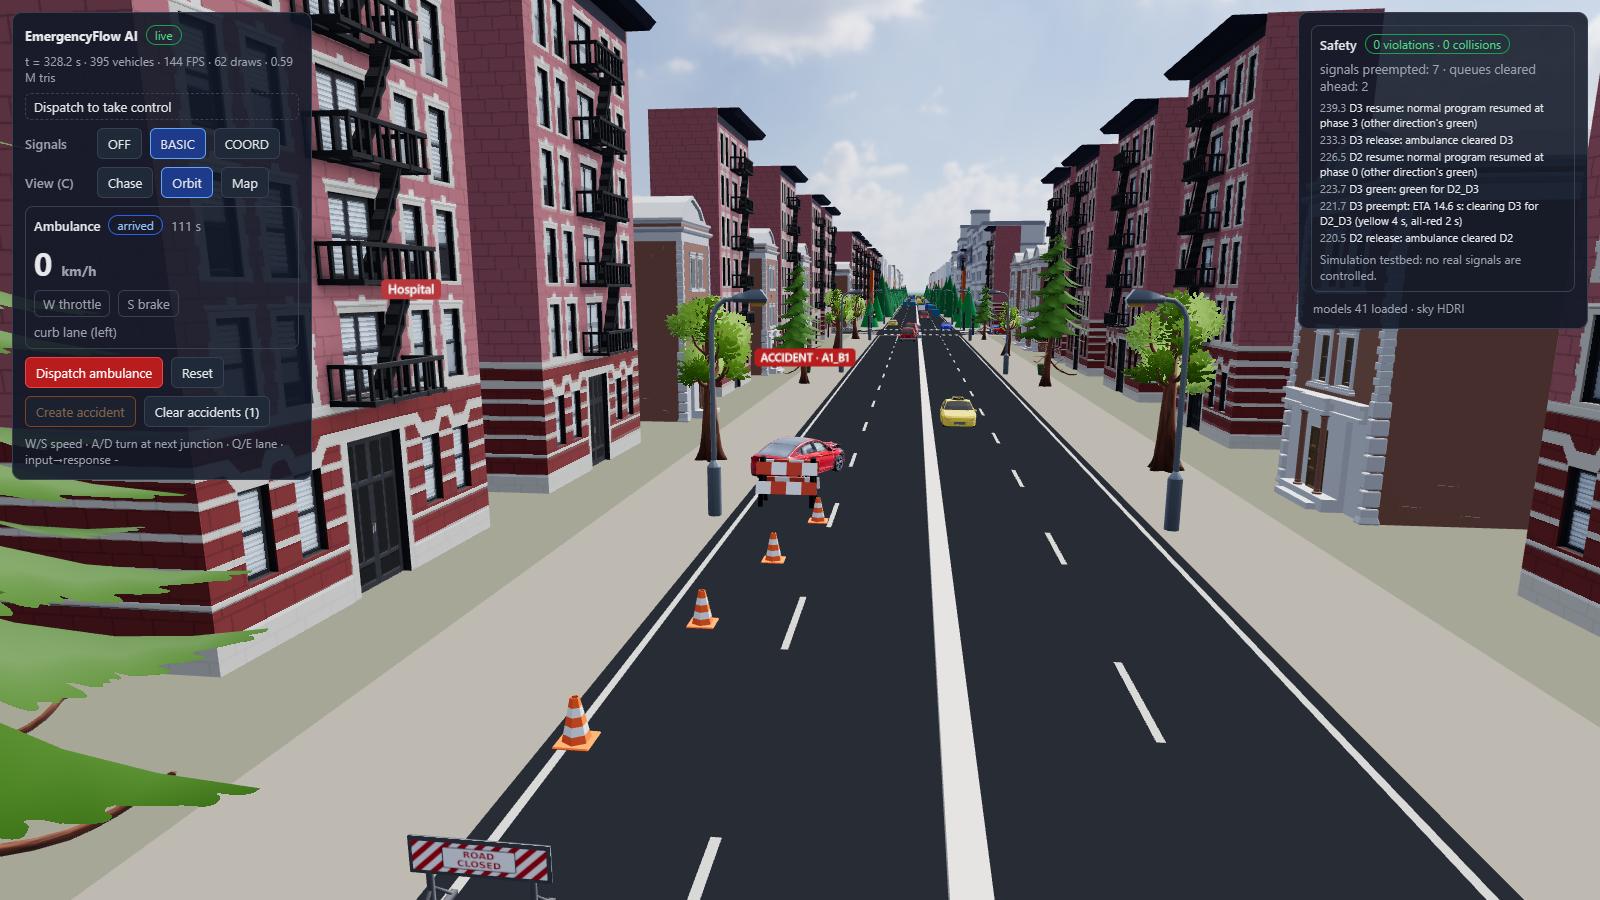
\includegraphics[width=\columnwidth]{accident_scene.png}
\caption{An injected accident: the wreck blocks the curb lane, a barrier and cone taper close it, and SUMO's traffic merges into the open lane.}
\label{fig:accident}
\end{figure}

\section{Evaluation Methodology}

\subsection{Arms}

We compare eight arms, three signal strategies plus a baseline variant crossed with two routing policies:
\begin{itemize}
\item \textbf{OFF strict}: normal signals; the ambulance obeys red lights.
\item \textbf{OFF realistic}: normal signals; the ambulance may cross a red light at up to 20\,km/h, modelled with SUMO's junction-model parameters for driving through red.
\item \textbf{BASIC} and \textbf{COORD} as described above.
\end{itemize}
Each strategy is run with \emph{static} routing (the free-flow route fixed at dispatch, as a map would give) and \emph{dynamic} routing (live re-planning). The baseline is OFF strict with static routing. In every run the ambulance is driven by an autopilot that follows the suggested route; every route change it makes is reviewed by the safety controller. The live demonstration is manual; all numbers in this paper are autopilot runs.

\subsection{Fair Baseline}

All arms share one fixed-time program tuned for the demand with SUMO's implementation of Webster's method \cite{webster}. One hour of demand is expanded into individual vehicles and passed to the tuning tool, which keeps the phase states, yellows and all-reds and changes only the green times. The tuned cycles were 27.9, 29.8, 34.7 and 36.2\,s on average at demands 0.75, 1.0, 1.5 and 2.0, against 74\,s in the generated network. The safety controller, the monitor and routing read the same program the simulator runs.

\subsection{Paired, Seeded Missions}

Each seed draws a dispatch time between 300 and 374\,s, so the signal phase at dispatch varies over one cycle, an origin on one side of the map and a destination on another, at least three quarters of the map's width apart. Every arm of a seed replays the same traffic up to the dispatch; a fingerprint of all vehicle positions and speeds at dispatch is stored per run and was identical across arms for every seed. The engine is deterministic: a replay reproduced a 243.5\,s mission with no differing position. Saved simulator states were tried as a shortcut and rejected, because a resumed run diverged at once, with five emergency brakings and a junction collision where the original had one braking and none. Each run continues for a fixed 600\,s after dispatch, so background metrics cover the same window, recovery included.

\subsection{Metrics and Statistics}

The primary metric is ambulance travel time from dispatch to arrival. Secondary metrics are waiting time, red-light stops, the time for the queue in front of the ambulance to clear at each junction, the mean queue per signalised approach, and the background time loss of all other vehicles from SUMO's trip information, written with unfinished trips at the end of the window. Because vehicles already on the road carry losses from before the dispatch, identical across arms, only paired differences are interpreted. Safety is counted from the monitor, SUMO's collision detection and its emergency-braking and teleport warnings. For each arm we report the mean paired difference to the baseline with a 95\,\% percentile bootstrap confidence interval \cite{efron,efron_book} (10{,}000 seeded resamples) and an exact two-sided Wilcoxon signed-rank $p$-value \cite{wilcoxon}, computed over all sign assignments with tied ranks. A run is excluded if the ambulance did not arrive within the window or any vehicle teleported after dispatch.

We ran 40 seeds at demand 1.5, the demonstration setting, and 10 seeds each at 0.75, 1.0 and 2.0: 560 runs in total. One run was excluded (an OFF realistic mission at demand 2.0 did not arrive within 600\,s); no run had a teleport.

\section{Results}

\subsection{Travel Time}

Table~\ref{tab:travel} lists mean travel times and Fig.~\ref{fig:sweep} the demand sweep with confidence bands. Preemption roughly halved the ambulance's travel time at every demand, and its benefit grew with congestion: the paired reduction against the baseline was 44\,s at demand 0.75, 60\,s at 1.0, 103\,s at 1.5 and 113 to 119\,s at 2.0 (all $p\le0.002$). With preemption the travel time stayed between 84 and 99\,s whatever the demand, while the baseline rose from 134 to 212\,s.

\begin{table}[t]
\caption{Mean Ambulance Travel Time (s), $4\times4$ Grid}
\begin{center}
\begin{tabular}{@{}lcccc@{}}
\toprule
\textbf{Arm} & \textbf{0.75} & \textbf{1.0} & \textbf{1.5} & \textbf{2.0} \\
\midrule
OFF strict, static (baseline) & 133.8 & 153.6 & 197.1 & 212.4 \\
OFF strict, dynamic & 123.9 & 161.0 & 195.6 & 179.7 \\
OFF realistic, static & 116.3 & 130.8 & 170.6 & 143.4 \\
OFF realistic, dynamic & 110.3 & 142.1 & 164.2 & 148.2 \\
BASIC, static & 89.7 & 93.2 & 93.8 & 99.2 \\
BASIC, dynamic & 84.3 & 91.4 & 95.9 & 93.6 \\
COORD, static & 89.4 & 93.7 & 94.6 & 95.8 \\
COORD, dynamic & 83.6 & 91.3 & 97.3 & 98.1 \\
\midrule
Seeds & 10 & 10 & 40 & 10 \\
\bottomrule
\end{tabular}
\label{tab:travel}
\end{center}
\end{table}

\begin{figure}[t]
\centering
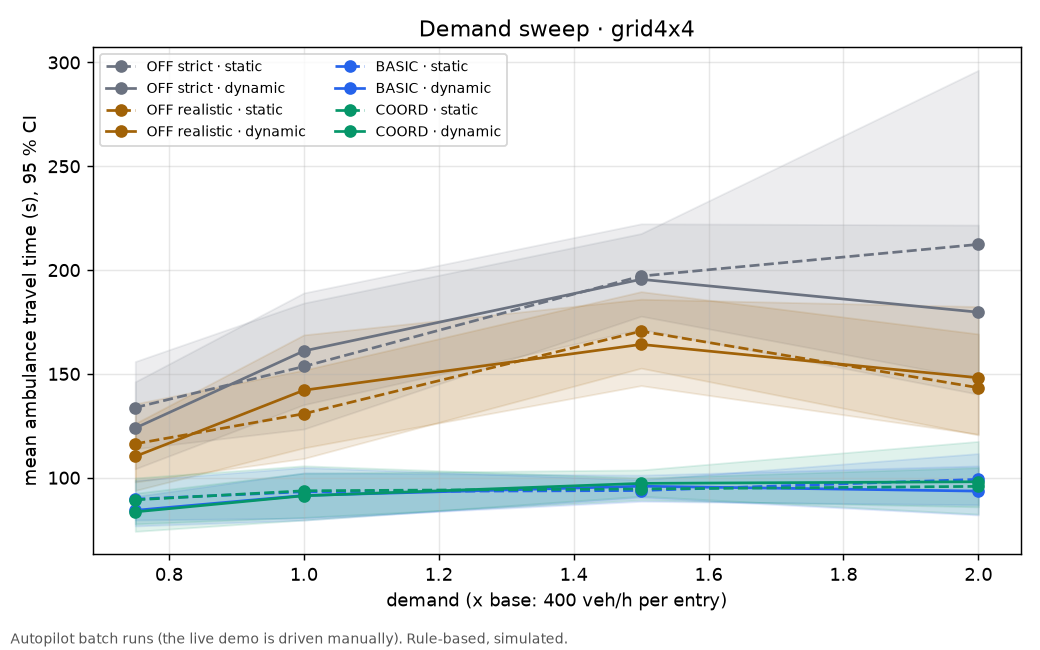
\includegraphics[width=\columnwidth]{demand_sweep.png}
\caption{Mean ambulance travel time against demand with 95\,\% bootstrap confidence bands (autopilot batch runs; dashed lines: static routing).}
\label{fig:sweep}
\end{figure}

Table~\ref{tab:paired} details the demonstration setting. With preemption the ambulance stopped at no red light, its waiting time fell from 56.5 to 0.1\,s, and the time for the queue in front of it to clear at each junction fell from 5.4 to 1.5\,s. Fig.~\ref{fig:dist} shows the per-seed distributions.

\begin{table*}[t]
\caption{Paired Differences Against the Baseline at Demand 1.5 (40 Seeds): Mean, 95\,\% Bootstrap CI, Exact Wilcoxon $p$}
\begin{center}
\begin{tabular}{@{}lcccc@{}}
\toprule
\textbf{Arm} & \textbf{Travel time (s)} & \textbf{Waiting time (s)} & \textbf{Red-light stops} & \textbf{Background time loss (veh$\cdot$s)} \\
\midrule
OFF strict, dynamic & $-1.6$ [$-23.3$, $19.4$], $p{=}0.99$ & $+5.5$ & $-0.3$ & $+11$ [$-478$, $469$], $p{=}0.98$ \\
OFF realistic, static & $-26.5$ [$-37.5$, $-16.7$], $p{<}0.001$ & $-24.1$ & $-1.1$ & $-89$ [$-442$, $300$], $p{=}0.38$ \\
OFF realistic, dynamic & $-32.9$ [$-54.5$, $-13.2$], $p{=}0.002$ & $-24.4$ & $-1.7$ & $-60$ [$-572$, $432$], $p{=}0.99$ \\
BASIC, static & $-103.3$ [$-121.9$, $-85.9$], $p{<}0.001$ & $-56.4$ & $-3.6$ & $+60$ [$-1064$, $1024$], $p{=}0.33$ \\
BASIC, dynamic & $-101.2$ [$-119.9$, $-83.7$], $p{<}0.001$ & $-56.4$ & $-3.6$ & $+330$ [$-955$, $1534$], $p{=}0.23$ \\
COORD, static & $-102.5$ [$-121.2$, $-85.3$], $p{<}0.001$ & $-56.4$ & $-3.6$ & $-184$ [$-1240$, $805$], $p{=}0.91$ \\
COORD, dynamic & $-99.8$ [$-118.1$, $-82.7$], $p{<}0.001$ & $-56.0$ & $-3.6$ & $+681$ [$-506$, $1821$], $p{=}0.17$ \\
\midrule
\multicolumn{5}{@{}l}{Baseline means: travel 197.1\,s, waiting 56.5\,s, 3.6 red-light stops, background time loss about 190{,}600 vehicle-seconds.}\\
\bottomrule
\end{tabular}
\label{tab:paired}
\end{center}
\end{table*}

\begin{figure}[t]
\centering
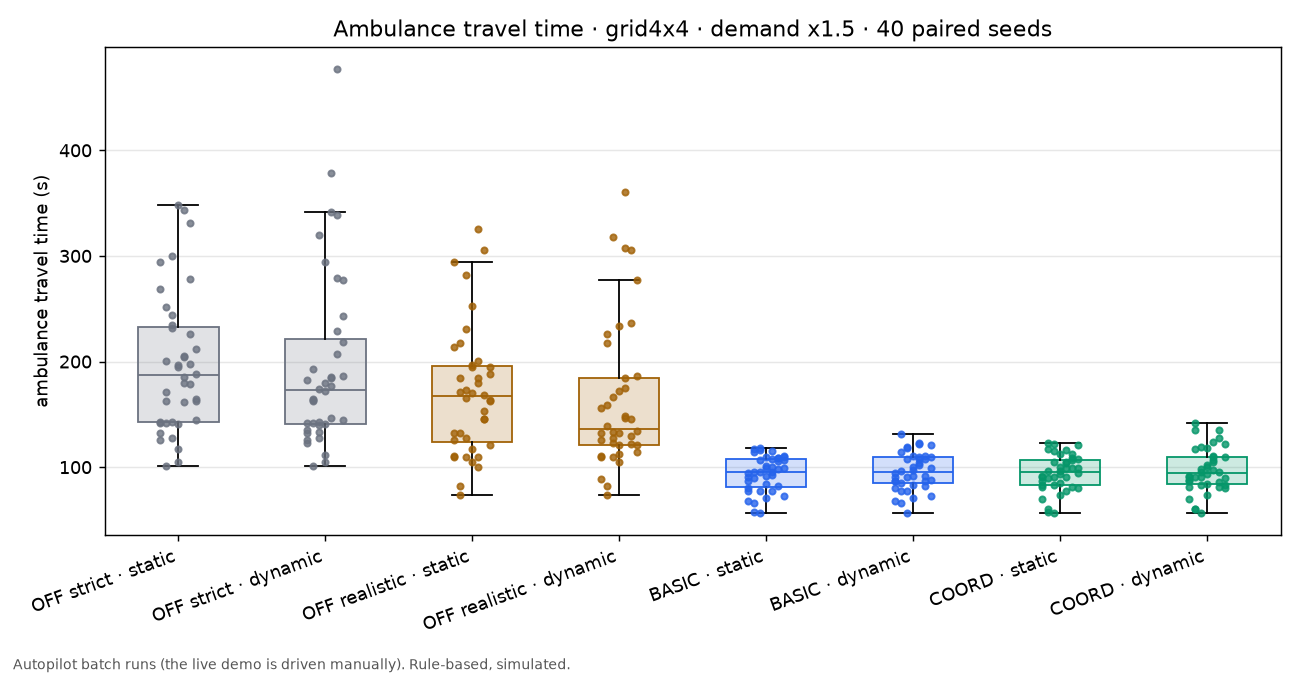
\includegraphics[width=\columnwidth]{travel_time_x1_5.png}
\caption{Per-seed ambulance travel times at demand 1.5 (40 paired seeds).}
\label{fig:dist}
\end{figure}

\subsection{Cost to Background Traffic}

The cost of preemption to other road users was not measurable. At every demand the paired change in total background time loss with BASIC or COORD stayed within $\pm0.7\,\%$ of the total and was never significant (Table~\ref{tab:paired}, Fig.~\ref{fig:bg}). We attribute this to the short tuned cycles: a preemption costs cross traffic one 6\,s clearance and part of a short green, after which recovery returns the junction to its program. The mean queue per signalised approach did not change significantly either.

\begin{figure}[t]
\centering
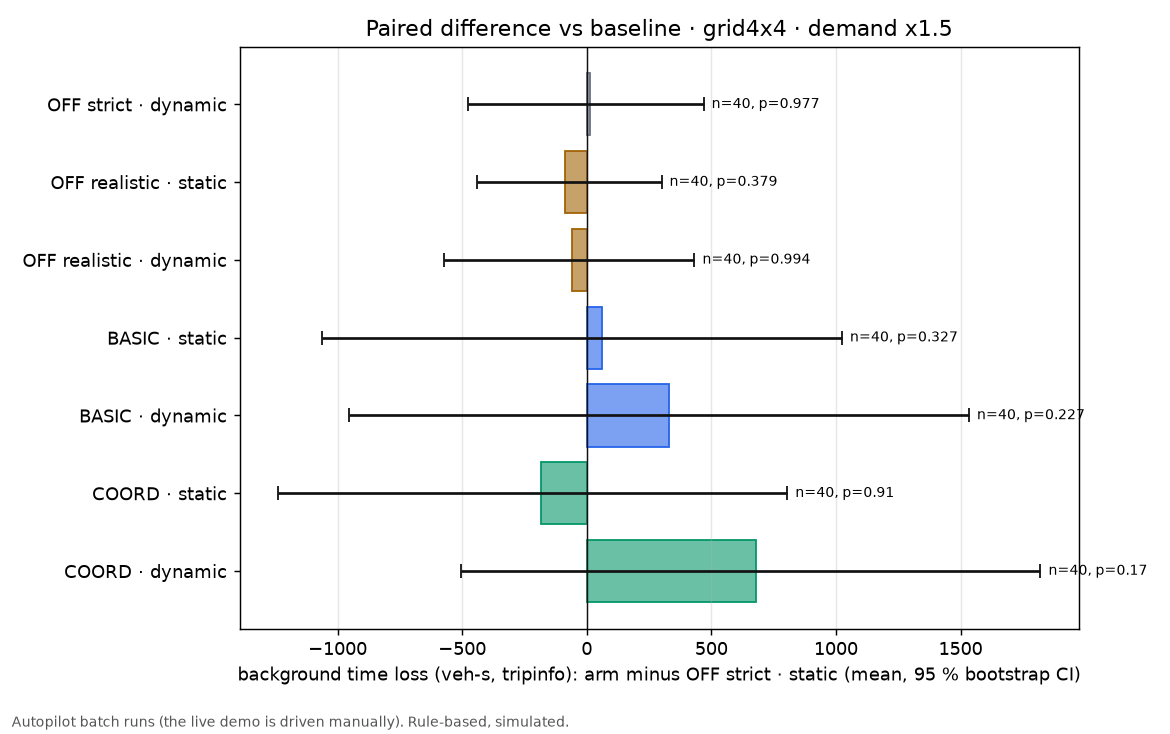
\includegraphics[width=\columnwidth]{background_delay_x1_5.png}
\caption{Paired change in background time loss against the baseline at demand 1.5, with 95\,\% bootstrap confidence intervals.}
\label{fig:bg}
\end{figure}

\subsection{Coordination and Re-Routing}

COORD was not better than BASIC. Table~\ref{tab:coord} lists the paired difference per demand; none was significant and all were under 5\,s. The tuned cycles of 28--36\,s leave short queues, so preparing junctions early has little to clear. In an earlier five-seed smoke test on the network's own 74\,s program, COORD was ahead of BASIC by 2 to 8\,s, which suggests that coordination pays off with long cycles and long queues; establishing this with paired runs is future work.

\begin{table}[t]
\caption{COORD Minus BASIC, Travel Time (s), Mean [95\,\% CI]}
\begin{center}
\begin{tabular}{@{}lcc@{}}
\toprule
\textbf{Demand} & \textbf{Static routing} & \textbf{Dynamic routing} \\
\midrule
0.75 & $-0.3$ [$-3.6$, $2.9$] & $-0.7$ [$-4.2$, $2.7$] \\
1.0 & $+0.5$ [$-1.7$, $3.5$] & $-0.1$ [$-2.0$, $1.8$] \\
1.5 & $+0.8$ [$-0.5$, $2.0$] & $+1.4$ [$-1.8$, $5.0$] \\
2.0 & $-3.4$ [$-8.4$, $0.5$] & $+4.5$ [$-3.7$, $18.4$] \\
\bottomrule
\multicolumn{3}{@{}l}{All $p\ge0.28$ (exact Wilcoxon).}
\end{tabular}
\label{tab:coord}
\end{center}
\end{table}

Live re-routing did not help without incidents either. With BASIC or COORD, dynamic and static routing differed by less than 6\,s at every demand, significantly only for COORD at demand 0.75 ($-5.8$\,s, $p=0.031$, ten seeds). On a regular grid without incidents the free-flow route is usually close to the best one, and once signals are preempted the main source of delay that routing could avoid is gone. The value of re-routing lies in incidents, where the testbed flags the compromised route and goes round the accident; the batch evaluation of accident scenarios is future work.

\subsection{Safety}

The independent monitor counted no violation of R1--R3 in any of the 560 runs. To attribute collisions, every run in which SUMO reported one was re-run with the simulator log kept; all 32 reproduced their collision counts exactly. Table~\ref{tab:safety} summarises the result. No collision involved the ambulance in any BASIC, COORD or OFF strict run (420 runs). The ambulance crossing red lights without priority was in a junction collision in 12 of the 140 OFF realistic runs (22 events): SUMO's red-crossing model does not yield to cross traffic, and the ambulance saved only 17 to 34\,s against the baseline. Preemption thus delivered between 2.5 and 4 times the saving of crossing red lights with no ambulance collision. The remaining collisions were between background vehicles at permissive turns, almost all at demand 2.0, where the network is oversaturated; they occurred in every arm, including the baseline.

\begin{table}[t]
\caption{Collision Events After Dispatch, Classified by Replay}
\begin{center}
\begin{tabular}{@{}lccc@{}}
\toprule
\textbf{Signals (both routings)} & \textbf{Runs} & \textbf{Events} & \textbf{With ambulance} \\
\midrule
OFF strict & 140 & 13 & 0 \\
OFF realistic & 140 & 36 & 22 \\
BASIC & 140 & 13 & 0 \\
COORD & 140 & 14 & 0 \\
\bottomrule
\multicolumn{4}{@{}l}{Signal-safety violations (monitor, R1--R3): 0 in all 560 runs.}
\end{tabular}
\label{tab:safety}
\end{center}
\end{table}

\subsection{Live Ghost Comparison}

The batch results compare policies; the interactive demonstration needs a measurement for the mission being driven. A shadow simulation starts with the live one, in its own process, with the same scenario, seed, demand and warm-up, and steps in lockstep with the live simulation time without an ambulance, so its traffic is the live traffic. At the first dispatch after a reset it sends out its own ambulance at the same simulated moment, driven by the autopilot under normal signals, and accidents injected live are mirrored at the same moment. When the live ambulance arrives, the shadow runs ahead to its own arrival and the difference is reported as the time saved, and its ambulance is drawn as a translucent ghost (Fig.~\ref{fig:live}). A test drives the live simulation exactly like the ghost and checks that both missions take identical times with identical positions, with and without an accident on the route. In one recorded demonstration at demand 1.5, a manually driven mission that switched from normal signals to BASIC and COORD and went round an injected accident arrived in 167\,s, against 212.6\,s for its ghost. This single example illustrates the mechanism; the evidence for the policies is the batch evaluation above.

\section{Implementation and Verification}

The engine is written in Python with FastAPI and talks to SUMO 1.27.1 through TraCI; the front end uses React, React Three Fiber and Three.js, renders the team's 3D models with instancing and level of detail, and runs in an ordinary browser. The whole system starts on a single laptop with one command and runs locally; a read-only dashboard can be opened from other computers on the same network.

Verification is part of the design rather than an afterthought. The backend has 143 automated tests and the front end 84, all passing at the time of writing. They cover, among others: the invariants R1--R3 on hand-built and generated plans, including the normal program over three cycles; the clearance timing as observed in the simulator, measured as the difference between observed switch times; emergency-class authorisation and the preemption timeout; the fail-safe when the decision logic throws; the dead-man timer with an injected clock; the speed cap; and a one-hour heavy-demand scenario that must finish without teleports or collisions. Architecture tests fail the build if a signal setter appears outside the traffic-light module, if the simulator client is imported outside the simulation layer, or if the decision or safety layers import the simulator, the API or the network library. A contract test generates example messages from the server's message models into the front end's type checker, so any field, command or enumeration that drifts between the two sides breaks the build.

Reproducibility is enforced at run level. Every run writes a manifest with the SUMO version, the source revision and whether the working tree was clean, a hash of the scenario files, simulator options, signal program, arm and window, and the seed, demand and mission. Batch runs are executed from a separate checkout pinned to a committed revision, so that edits made during a long batch cannot leak into it. The determinism of the engine is itself tested: the ghost comparison must report a time saved of exactly zero, with identical positions, when the live mission is driven like the ghost. The statistical code is tested against full enumeration of sign assignments for the Wilcoxon test.

\section{Discussion and Limitations}

The results are strongest for the effect that matters most: preemption with verified clearance gives a large, consistent reduction in travel time at no measurable cost to other traffic, on a fairly tuned baseline. The negative results are equally informative. Coordination and live re-routing added nothing measurable on a regular grid without incidents, and a testbed that reports this honestly is more useful than one that only confirms its own features.

Several limitations apply. The network is a synthetic grid; real cities have irregular geometry, unequal approaches and actuated signals. Background traffic consists of passenger cars only, because buses and trucks on permissive turns caused simulator junction collisions; they require protected turn phases. The red-crossing baseline depends on SUMO's model, which does not yield; a more cautious model would likely avoid some collisions and change that comparison. Background collisions at demand 2.0 indicate the limits of permissive turning under oversaturation in the simulator. Experiments use an autopilot; human drivers in the live mode behave differently. Finally, the testbed controls only simulated signals.

\subsection{Path to Field Deployment}

The testbed is intended as a step towards deployment in Navi Mumbai rather than a substitute for it, and several elements would have to be added and validated before any field use. Vehicle detection is idealised here: the simulator knows the ambulance's exact position, next signal and lane link, whereas a field system needs positioning and communication between the vehicle and the junction, with their latency and failure modes. The safety controller's checks would have to run on, or be enforced by, the junction controller itself, since a field controller has its own conflict monitoring and minimum timings that must remain authoritative; the invariants R1--R3 correspond to the kind of checks such hardware performs, but the mapping must be certified for each controller type. Real networks need calibrated demand, actuated and coordinated base programs, pedestrian phases and mixed traffic, including two-wheelers and auto-rickshaws, which the current simulation does not model. The testbed is useful in this process precisely because a candidate strategy, a local network and its demand can be evaluated with the same paired protocol before any equipment is installed, and because the cost to other road users is reported alongside the benefit to the ambulance.

\section{Conclusion and Future Work}

EmergencyFlow couples a microscopic traffic simulator, a rule-based decision layer, a doubly verified safety layer and an interactive 3D view into a closed loop, and evaluates strategies on paired, seeded traffic against a demand-tuned baseline. On 560 runs, preemption halved ambulance travel time at no measurable background cost and with no safety violation, crossing red lights saved less and caused collisions, and coordination and re-routing showed no gain without incidents. Future work includes batch evaluation of accident scenarios, paired experiments on long-cycle programs where coordination may matter, irregular networks imported from real city maps, heavy vehicles with protected turn phases, and several emergency vehicles at once.

\section*{Acknowledgment}

This work is supported by the Navi Mumbai Municipal Corporation (NMMC), IAS Administration. The authors thank Shri Ganesh Naik, MLA, Airoli Assembly Constituency, and Smt. Manda Vijay Mhatre, MLA, Belapur Assembly Constituency, for acknowledging the project, which has been proposed to the Mumbai Metropolitan Region Development Authority (MMRDA) for further development and implementation across the Navi Mumbai region.

\begin{thebibliography}{00}
\bibitem{fhwa_evp} U.S. Department of Transportation, Federal Highway Administration, ``Traffic signal preemption for emergency vehicles: A cross-cutting study,'' Rep. FHWA-JPO-05-010, Washington, DC, 2006.
\bibitem{mutcd} U.S. Department of Transportation, Federal Highway Administration, \emph{Manual on Uniform Traffic Control Devices for Streets and Highways}, 2009 ed. Washington, DC, 2009.
\bibitem{webster} F. V. Webster, ``Traffic signal settings,'' Road Research Laboratory, London, Road Research Tech. Paper no.~39, 1958.
\bibitem{sumo} P. A. Lopez \emph{et al.}, ``Microscopic traffic simulation using SUMO,'' in \emph{Proc. 21st IEEE Int. Conf. Intelligent Transportation Systems (ITSC)}, 2018, pp. 2575--2582.
\bibitem{traci} A. Wegener, M. Pi\'{o}rkowski, M. Raya, H. Hellbr\"{u}ck, S. Fischer, and J.-P. Hubaux, ``TraCI: An interface for coupling road traffic and network simulators,'' in \emph{Proc. 11th Communications and Networking Simulation Symp. (CNS)}, 2008, pp. 155--163.
\bibitem{krauss} S. Krau\ss, ``Microscopic modeling of traffic flow: Investigation of collision free vehicle dynamics,'' Ph.D. dissertation, Univ. of Cologne, Cologne, Germany, 1998.
\bibitem{erdmann} J. Erdmann, ``SUMO's lane-changing model,'' in \emph{Modeling Mobility with Open Data}, M. Behrisch and M. Weber, Eds. Cham: Springer, 2015, pp. 105--123.
\bibitem{dijkstra} E. W. Dijkstra, ``A note on two problems in connexion with graphs,'' \emph{Numerische Mathematik}, vol. 1, pp. 269--271, 1959.
\bibitem{wilcoxon} F. Wilcoxon, ``Individual comparisons by ranking methods,'' \emph{Biometrics Bulletin}, vol. 1, no. 6, pp. 80--83, 1945.
\bibitem{efron} B. Efron, ``Bootstrap methods: Another look at the jackknife,'' \emph{The Annals of Statistics}, vol. 7, no. 1, pp. 1--26, 1979.
\bibitem{efron_book} B. Efron and R. J. Tibshirani, \emph{An Introduction to the Bootstrap}. New York: Chapman \& Hall, 1993.
\end{thebibliography}

\end{document}
